\documentclass[a4paper,10pt,twocolumn,uplatex]{jsarticle}
\usepackage{style/nislab}
\usepackage{tabularx}

%---------------------------------------------------------------------
% レジュメ種別・日付設定(要変更)
% \type{} 1:修士論文諮問会 2:卒業論文発表会 else:月例発表会
\type{3}
\year{2021}
\month{8}
\date{11}

%---------------------------------------------------------------------
% ページ番号設定(要変更)
\setcounter{page}{3}

%---------------------------------------------------------------------
\begin{document}
%---------------------------------------------------------------------
% タイトル作成部分(要変更)
% \maketitle{タイトル}{title}{名前}{name}
\maketitle{IoTアプリケーションの使用頻度を考慮したSDNによる通信制御手法}
{A Method of SDN Based Communication Management Considering Frequency of IoT Application Use}
{国本 典晟}
{Tensei Kunimoto}

%---------------------------------------------------------------------
\section{はじめに}
近年,画像や動画などの大容量データの需要が急速に拡大したことによるインターネット全体の帯域の逼迫が問題になっているが,IoTデバイスの増加とスマートホームの技術の進歩に伴い,ホームネットワーク内部の帯域並びにホームネットワーク外部のインターネットの帯域の逼迫はより深刻化すると予想される.現在,ISP (Internet Service Provider) は各家庭の総帯域を契約した帯域の範囲内で制御しており,要求される帯域が回線の帯域を上回る場合、特定アプリケーションやユーザの帯域を制御することでネットワークの品質確保に努めている.しかし,そういった帯域制御は多様なサービスやトラフィックに最適化されたものではなく,IoTデバイスが要求する複数のQoS要件を満たすことができない.\par
この問題の解決を目指して,IoTデバイスのサービスカテゴリごとに適切な帯域を割り当てる管理アーキテクチャが提案されているが,複数のQoS要件を満たすためのアルゴリズムが課題になっている.本研究では,アプリケーションの使用頻度を考慮したIoTデバイス管理アーキテクチャの実装と評価を行う.\par

%---------------------------------------------------------------------
\section{関連研究}

%---------------------------------------------------------------------
\subsection{SDNベースのQoSを考慮した帯域管理フレームワーク}
Jangらは,スマートホームのネットワークデバイスのための革新的なネットワーク管理モデルを開発する必要があるとして,SDNベースのQoSを考慮した帯域管理フレームワークを提案した\cite{framework}.この研究では,QCI (3GPP LTE QoS Class Identifier) をスマートホーム向けのサービス用に\tabref{tab:QCI}のように再定義し,QCIサービスをパケット遅延の上限値に基づいて「高優先度クラス」「中優先度クラス」「低優先度クラス」の3つに分類することで各サービスのQoSの最適化を目指した.実験の結果,従来のISPの帯域制御手法を上回る結果を得た.\par

\newcolumntype{A}{>{\centering\arraybackslash}p{3mm}}
\newcolumntype{B}{>{\centering\arraybackslash}p{7mm}}
\newcolumntype{C}{>{\centering\arraybackslash}p{8mm}}
\begin{table}[!bt]
  \caption{スマートホームサービス向けに再定義されたQCI}
  \label{tab:QCI}
  \centering
  {\scriptsize
  \begin{tabularx}{\linewidth}{ABBCCBX}
    \hline
    QCI & Priority & Device type & Resource Type & Packet Delay Budget & Packet Error Loss & \multicolumn{1}{c}{Example Services}\\
    \hline \hline
    1 & 2 & Non-M2M & GBR & 100ms & $10^{-2}$ & Conversational voice\\
    2 & 3 & Non-M2M & GBR & 50ms & $10^{-3}$ & Real time gaming\\
    3 & 4 & Non-M2M & GBR & 150ms & $10^{-3}$ & Conversational video\\
    4 & 5 & Non-M2M & GBR & 300ms & $10^{-6}$ & Non-conversational video (Buffered streaming)\\
    5 & 1 & M2M & Non-GBR & 60ms & $10^{-6}$ & Mission critical delay sensitive data transfer\\
    6 & 6 & Non-M2M & Non-GBR & 300ms & $10^{-6}$ & Video (Buffered streaming) TCP-based (for example,www,email,chat,ftp,p2p and the like)\\
    7 & 7 & Non-M2M & Non-GBR & 100ms & $10^{-3}$ & Voice,Video (Live streaming),Interactive gaming\\
    8 & 8 & M2M & Non-GBR & N/A & $10^{-6}$ & Non mission critical delay insensitive data transfer\\
    \hline
  \end{tabularx}
  }
\end{table}

%---------------------------------------------------------------------
\subsection{AQRA}
Dengらは,Jangらが提案したスマートホーム向けに再定義したQCIを利用して,AQRA (Application-aware QoS Routing Algorithm) を提案した\cite{AQRA}.AQRAでは,複数のQoS要件を満たすフローの最適な経路の選択をSAアルゴリズムにより行った.また,高優先度クラスに属するアプリケーションのQoS要件の不満足を防ぐために,QoSを考慮したアドミッション制御を提案した.実験の結果,QoSを考慮したアドミッション制御を行ったAQRAは,行わなかったAQRAと比較して高優先度クラスに属するアプリケーションのQoSの適合率は向上した一方で,中優先度クラス及び低優先度クラスに属するアプリケーションのQoSの適合率は低下した.\par

%---------------------------------------------------------------------
\section{提案手法}

%---------------------------------------------------------------------
\subsection{概要}
これまで提案された帯域管理システムでは,QCIのリソースタイプのに応じてアプリケーションを「高優先度クラス」「中優先度クラス」「低優先度クラス」の3つのクラスに分類していた.高優先度クラスに属するのはガスセンサや侵入者アラームなどの非リアルタイムかつ遅延の許されないアプリケーションであり,中優先度クラスに属するのは映像データや音声データなど,遅延制限が厳しいリアルタイムサービスのアプリケーションである,低優先度クラスの属するのは遅延の許されるアプリケーションである.高優先度クラスに属するアプリケーションは必要時には十分な帯域が確保されるべきであるが,スマートホームのユーザの使用頻度は中優先度クラス及び低優先度クラスのアプリケーションの方が高く,常に高優先度クラスのアプリケーションのために中優先度クラス及び低優先度クラスの帯域が犠牲になるのはQoEを著しく損なう.本研究では,\cite{AQRA}で提案されたQoSを考慮したアドミッション制御の見直しを行うとともに,アプリケーションの動作状態に応じてアドミッション制御の切り替えを行い,ユーザのアプリケーションの使用頻度を考慮した通信制御を行う.

%---------------------------------------------------------------------
\subsection{実験環境}
本研究で想定するアーキテクチャを図\ref{fig:Architecture}に示す.\par
前提条件は以下の通りである.\par

\begin{itemize}
  \item IoTアプリケーション・サービスはイーサネットを介してネットワーク層に接続している.
  \item IoTアプリケーションはNorthbound APIを介してSDNコントローラにメッセージを送信できる.
  \item SDNスイッチ間はイーサネットで接続されている.
  \item SDNスイッチはSouthbound APIを介してSDNコントローラと通信できる.
  \item SDNスイッチとIoTゲートウェイはイーサネットで接続されている.
  \item IoTゲートウェイとIoTデバイスは無線通信技術で接続されている.
\end{itemize}

\begin{figure}[!tb]
  \centering
  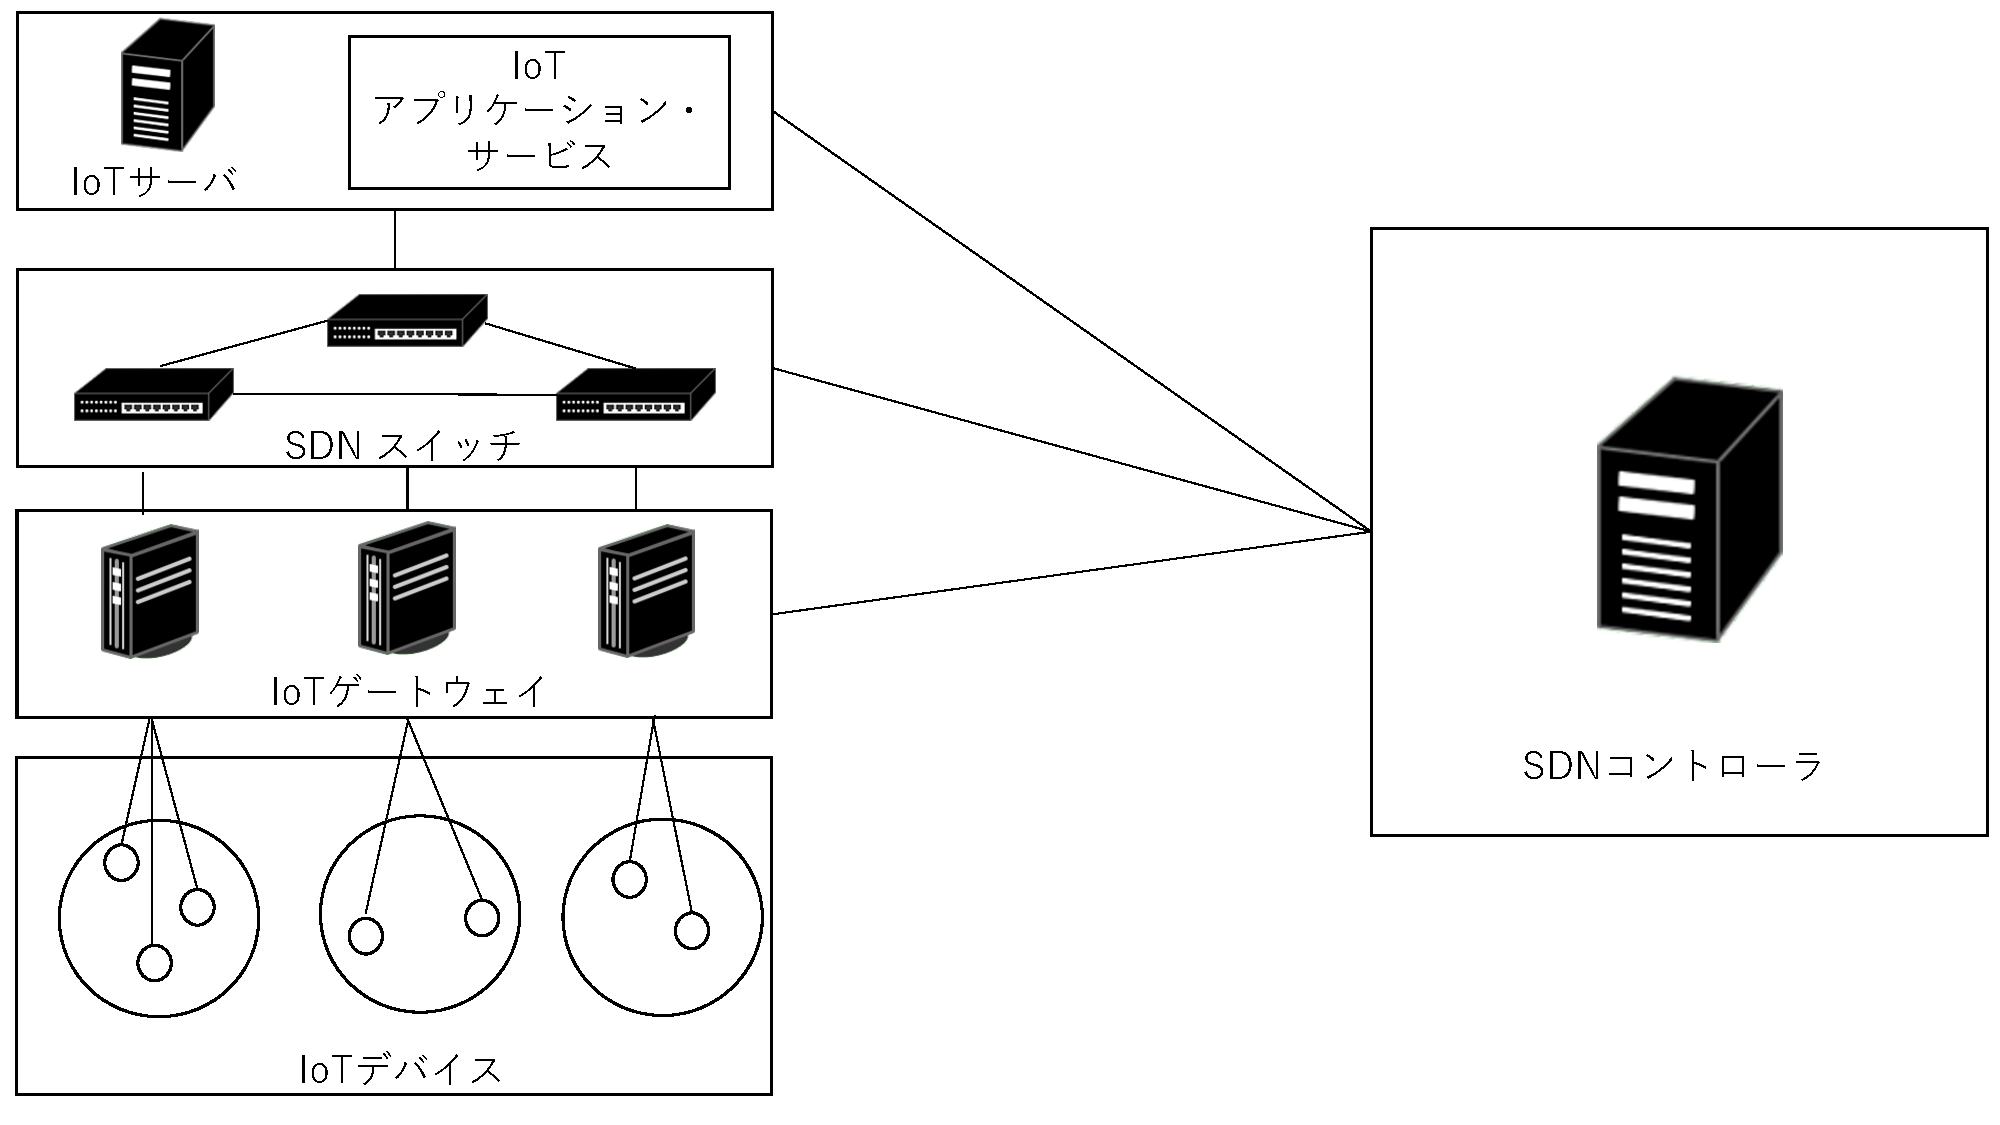
\includegraphics[width=\linewidth]{img/AQRA_Architecture.pdf}
  \caption{提案システムのアーキテクチャ}
  \label{fig:Architecture}
\end{figure}

%---------------------------------------------------------------------
\subsection{動作手順}
動作手順を以下に示す.

\begin{enumerate} % 箇条書きは \begin{itemize}
  \item 各IoTアプリケーションはIoTアプリケーションサーバのIPアドレスとともにQCIをSDNコントローラに送信する.
  \item IoTゲートウェイはIoTデバイスからデータフローを受信すると,SDNコントローラにPacket Inメッセージを送信する.
  \item SDNコントローラはPacket Inメッセージを受信すると以下の作業を実行する.
  \item SDNコントローラはQCIに従いフローを分類する.
  \item SDNコントローラはルーティングパスを計算しフローエントリを設定する.
  \item SDNコントローラはQoSを考慮したアドミッション制御をIoTゲートウェイに送信し,優先度の低いIoTアプリケーションのアドミッションを制御する.
\end{enumerate}

%---------------------------------------------------------------------
\section{評価}

%---------------------------------------------------------------------
\subsection{評価方法}
本研究で提案する帯域管理システムはQoSが向上することを目的とするため,評価は平均転送率,平均ジッタ,平均遅延時間の測定により行う.その際,高優先度クラスのアプリケーションのサービスが必要となった時は高優先度クラスのアプリケーションのQoS要件を保証するが,平常時はアプリケーションの使用頻度を考慮して,中優先度クラス及び低優先度クラスのQoS要件を保証できているかを評価する.また,提案システムが膨大な数のスマートホームの管理を行った際に目的の通りQoSを保証できるかを確認するため,システムが管理するスマートホームとIoTデバイスの数が増加した場合の平均転送率,平均ジッタ,平均遅延時間の変化を評価する.\par

%---------------------------------------------------------------------
\subsection{評価環境}
評価環境を以下に示す.\par

\begin{itemize}
  \item SDNコントローラにはOpenDaylight Neonを用いる.
  \item エミュレータにはMininetを用いる.
  \item IoTデバイスは30台〜100台で変化させる.
  \item 高優先度クラスのフローは30%とする.
  \item 中優先度クラスのフローは40%とする.
  \item 低優先度クラスのフローは30%とする.
\end{itemize}

%---------------------------------------------------------------------
\section{まとめと今後の課題}
本研究では,\cite{AQRA}で提案されたQoSを考慮したアドミッション制御の見直しと切り替えを行うことで,アプリケーションの使用頻度を考慮した通信制御を行い,帯域の効率的な活用及びスマートホームのサービスの複数のQoS要件の満足を目的とする.\par
今後の課題として,QoSを考慮したアドミッション制御の具体的な改善案や,アドミッション制御の切り替えの基準を考える必要がある.\par

%---------------------------------------------------------------------
% Bibliography
\footnotesize{
  \begin{thebibliography}{99}
    \bibitem{framework} Hung-Chin Jang and Jian-Ting Lin,SDN Based QoS Aware Bandwidth Management Framework of ISP for Smart Homes,2017 IEEE SmartWorld/SCALCOM/UIC/ATC/CBDCom/IOP/SCI,2017/8
    \bibitem{AQRA} Guo-Cin Deng and Kuochen Wang,An Application-aware QoS Routing Algorithm for SDN-based IoT Networking,2018 IEEE ISCC,p186-191,2018/6
  \end{thebibliography}
}

%---------------------------------------------------------------------
\end{document}
%---------------------------------------------------------------------
